\documentclass[11pt,a4paper]{article}
\usepackage[utf8]{inputenc}
\usepackage[T1]{fontenc}
\usepackage[margin=2cm]{geometry}
\usepackage{xcolor}
\usepackage{tikz}
\usetikzlibrary{shapes.geometric, arrows.meta, positioning, fit, backgrounds}
\usepackage{graphicx}
\usepackage{enumitem}
\usepackage{parskip}

\definecolor{navy}{HTML}{002155}
\definecolor{gold}{HTML}{FD9923}
\definecolor{light}{HTML}{F4F6FA}
\definecolor{green}{HTML}{0B6B2E}
\definecolor{amber}{HTML}{B77A2F}

\tikzset{
  box/.style={rectangle, draw=navy, fill=light, text=navy, rounded corners=2pt, align=center, minimum height=8mm, font=\small, inner sep=4pt},
  goldbox/.style={rectangle, draw=amber, fill=white, rounded corners=2pt, align=center, minimum height=8mm, font=\small, inner sep=4pt},
  decision/.style={diamond, draw=amber, fill=white, align=center, font=\small, inner sep=1pt, aspect=2.4},
  start/.style={rectangle, draw=green, fill=white, rounded corners=8pt, align=center, font=\small\bfseries, minimum height=8mm, inner sep=5pt},
  end/.style={rectangle, draw=navy, fill=navy!10, rounded corners=8pt, align=center, font=\small\bfseries, minimum height=8mm, inner sep=5pt},
  arrow/.style={-{Stealth[length=2.4mm]}, thick, color=navy},
  entity/.style={rectangle, draw=navy, fill=white, text=navy, align=center, font=\footnotesize\bfseries, minimum height=7mm, inner sep=3pt},
  rel/.style={draw=amber, thick},
}

\newcommand{\flowtitle}[1]{{\color{navy}\large\bfseries #1}}

\begin{document}

% ─────────────────────────────────────────────────────────────
\begin{center}
{\color{navy}\fontsize{26}{30}\selectfont\bfseries SIH 2026 --- Hackathon Platform}\\[2mm]
{\color{gold}\large Flow of Every Implemented Feature}\\[1mm]
{\color{navy!70}\normalsize TCET Centre of Excellence for Research Culture \& Development}
\end{center}
\vspace{2mm}

\noindent\rule{\textwidth}{0.6pt}
{\small This document traces the complete journey of every role on the portal --- \textbf{Student}, \textbf{Coordinator (admin)} and \textbf{Judge} --- through the system built for the SIH 2026 internal hackathon: registration with UID auto-derivation, venue and judge management, multi-round rubric judging with comments and overrides, notices, feedback and media.}

\section*{1. Actors and Modules}
\begin{center}
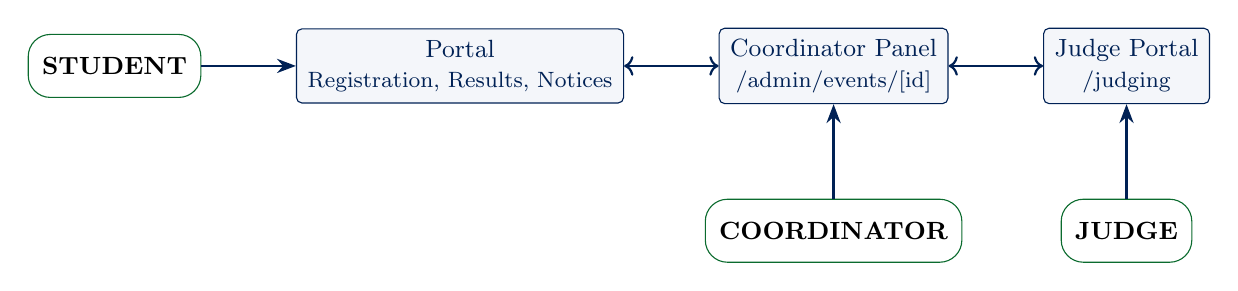
\begin{tikzpicture}[node distance=14mm]
  \node[start] (s) {STUDENT};
  \node[box, right=12mm of s] (portal) {Portal\\\footnotesize Registration, Results, Notices};
  \node[box, right=12mm of portal] (coord) {Coordinator Panel\\\footnotesize /admin/events/[id]};
  \node[box, right=12mm of coord] (judge) {Judge Portal\\\footnotesize /judging};
  \node[start, below=12mm of coord] (c) {COORDINATOR};
  \node[start, below=12mm of judge] (j) {JUDGE};
  \draw[arrow] (s) -- (portal);
  \draw[arrow] (c) -- (coord);
  \draw[arrow] (j) -- (judge);
  \draw[arrow, <->] (coord) -- (portal);
  \draw[arrow, <->] (judge) -- (coord);
\end{tikzpicture}
\end{center}

\section*{2. Event Lifecycle}
\begin{center}
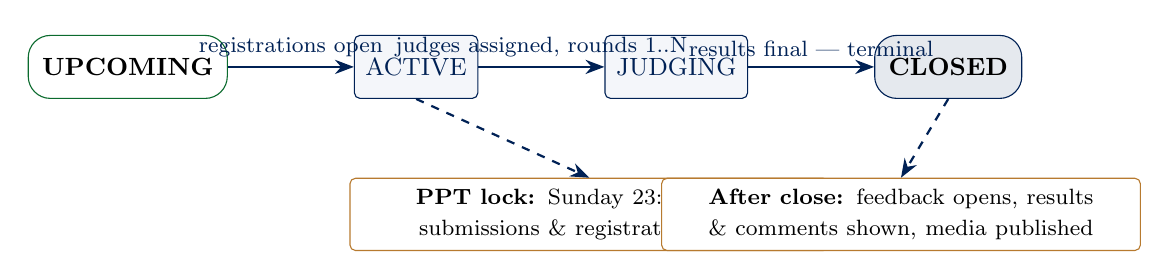
\begin{tikzpicture}[node distance=16mm]
  \node[start] (up) {UPCOMING};
  \node[box, right=16mm of up] (act) {ACTIVE};
  \node[box, right=16mm of act] (judging) {JUDGING};
  \node[end, right=16mm of judging] (closed) {CLOSED};
  \draw[arrow] (up) -- node[above, font=\footnotesize]{registrations open} (act);
  \draw[arrow] (act) -- node[above, font=\footnotesize]{judges assigned, rounds 1..N} (judging);
  \draw[arrow] (judging) -- node[above, font=\footnotesize]{results final --- terminal} (closed);
  \node[goldbox, below=10mm of act, xshift=22mm, text width=58mm] (lock) {\footnotesize \textbf{PPT lock:} Sunday 23:59:59 IST\\ submissions \& registration freeze};
  \node[goldbox, below=10mm of closed, xshift=-6mm, text width=58mm] (fb) {\footnotesize \textbf{After close:} feedback opens, results \& comments shown, media published};
  \draw[arrow, dashed] (act.south) -- (lock.north);
  \draw[arrow, dashed] (closed.south) -- (fb.north);
\end{tikzpicture}
\end{center}

\section*{3. Student --- Registration Flow}
\begin{center}
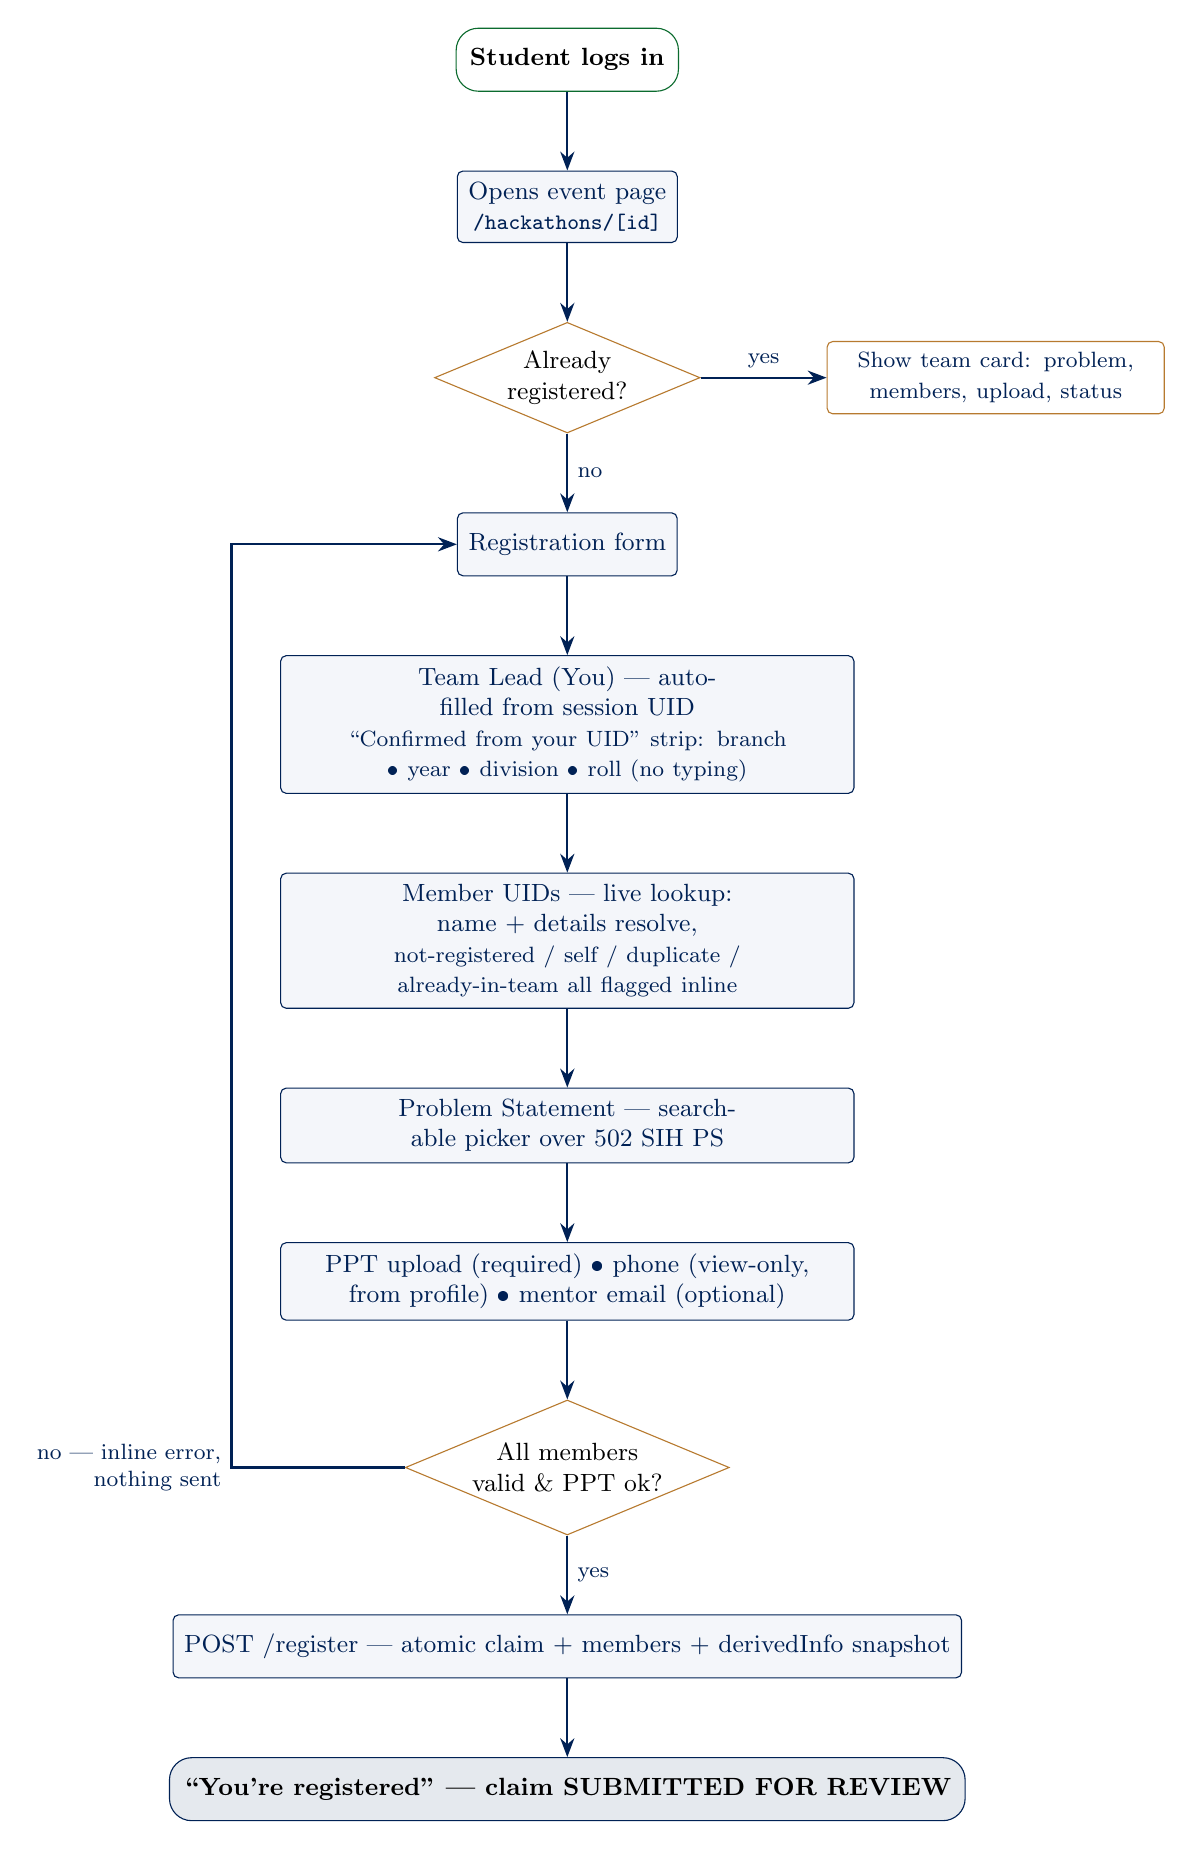
\begin{tikzpicture}[node distance=13mm]
  \node[start] (login) {Student logs in};
  \node[box, below=10mm of login] (open) {Opens event page\\\footnotesize \texttt{/hackathons/[id]}};
  \node[decision, below=10mm of open] (reg) {Already\\registered?};
  \node[box, below=10mm of reg] (form) {Registration form};
  \node[box, below=10mm of form, text width=70mm] (derive) {Team Lead (You) --- auto-filled from session UID\\\footnotesize ``Confirmed from your UID'' strip: branch \textbullet\ year \textbullet\ division \textbullet\ roll (no typing)};
  \node[box, below=10mm of derive, text width=70mm] (members) {Member UIDs --- live lookup: name + details resolve, \\\footnotesize not-registered / self / duplicate / already-in-team all flagged inline};
  \node[box, below=10mm of members, text width=70mm] (ps) {Problem Statement --- searchable picker over 502 SIH PS};
  \node[box, below=10mm of ps, text width=70mm] (extra) {PPT upload (required) \textbullet\ phone (view-only, from profile) \textbullet\ mentor email (optional)};
  \node[decision, below=10mm of extra] (valid) {All members\\valid \& PPT ok?};
  \node[box, below=10mm of valid] (submit) {POST /register --- atomic claim + members + derivedInfo snapshot};
  \node[end, below=10mm of submit] (done) {``You're registered'' --- claim SUBMITTED FOR REVIEW};
  \draw[arrow] (login) -- (open);
  \draw[arrow] (open) -- (reg);
  \draw[arrow] (reg) -- node[right, font=\footnotesize]{no} (form);
  \draw[arrow] (form) -- (derive);
  \draw[arrow] (derive) -- (members);
  \draw[arrow] (members) -- (ps);
  \draw[arrow] (ps) -- (extra);
  \draw[arrow] (extra) -- (valid);
  \draw[arrow] (valid) -- node[right, font=\footnotesize]{yes} (submit);
  \draw[arrow] (submit) -- (done);
  \draw[arrow] (valid.west) -- ++(-22mm,0) node[left, font=\footnotesize, align=right]{no --- inline error,\\ nothing sent} |- (form.west);
  \node[box, right=16mm of reg, goldbox, text width=40mm] (already) {\footnotesize Show team card: problem, members, upload, status};
  \draw[arrow] (reg) -- node[above, font=\footnotesize]{yes} (already);
\end{tikzpicture}
\end{center}

\section*{4. Coordinator Flow}
\begin{center}
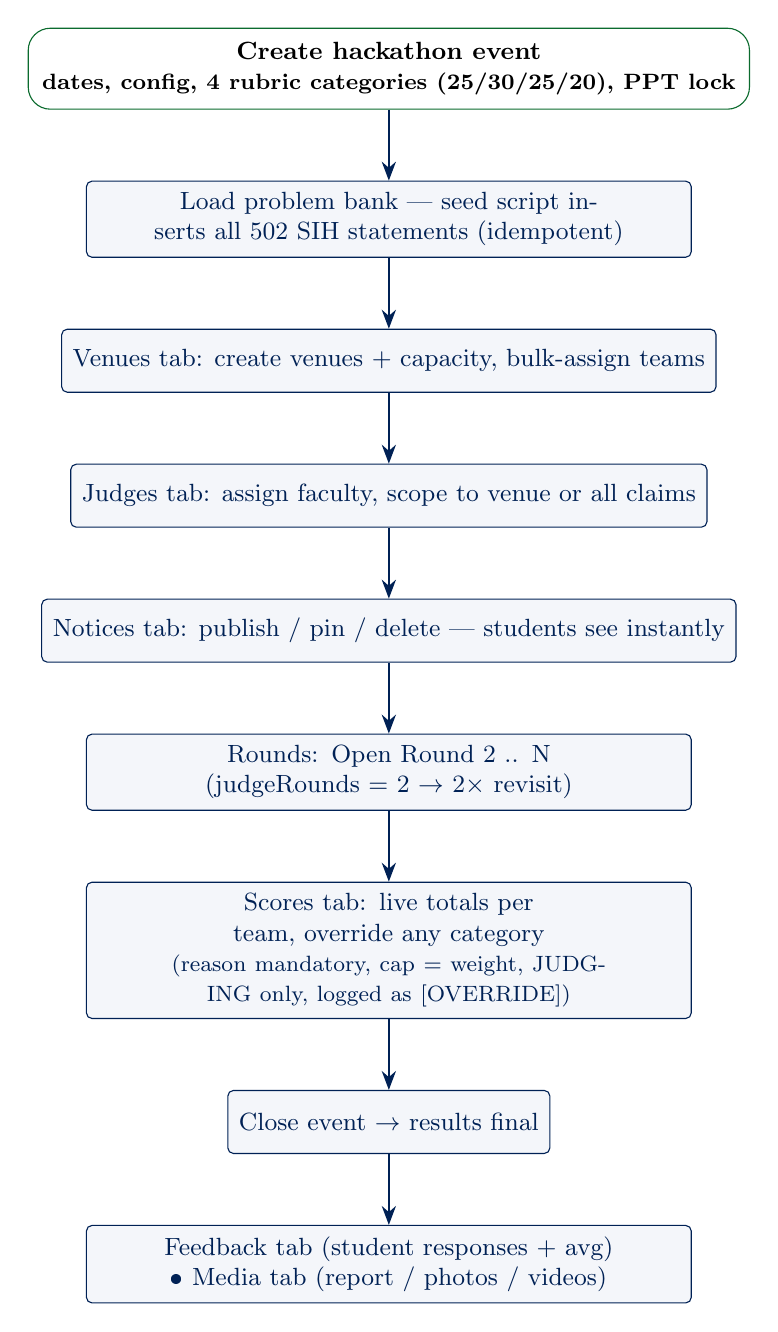
\begin{tikzpicture}[node distance=13mm]
  \node[start] (create) {Create hackathon event\\\footnotesize dates, config, 4 rubric categories (25/30/25/20), PPT lock};
  \node[box, below=9mm of create, text width=74mm] (load) {Load problem bank --- seed script inserts all 502 SIH statements (idempotent)};
  \node[box, below=9mm of load] (venues) {Venues tab: create venues + capacity, bulk-assign teams};
  \node[box, below=9mm of venues] (judges) {Judges tab: assign faculty, scope to venue or all claims};
  \node[box, below=9mm of judges] (notices) {Notices tab: publish / pin / delete --- students see instantly};
  \node[box, below=9mm of notices, text width=74mm] (rounds) {Rounds: Open Round 2 .. N (judgeRounds = 2 $\rightarrow$ 2$\times$ revisit)};
  \node[box, below=9mm of rounds, text width=74mm] (scores) {Scores tab: live totals per team, override any category\\\footnotesize (reason mandatory, cap = weight, JUDGING only, logged as [OVERRIDE])};
  \node[box, below=9mm of scores] (close) {Close event $\rightarrow$ results final};
  \node[box, below=9mm of close, text width=74mm] (wrap) {Feedback tab (student responses + avg) \textbullet\ Media tab (report / photos / videos)};
  \draw[arrow] (create) -- (load);
  \draw[arrow] (load) -- (venues);
  \draw[arrow] (venues) -- (judges);
  \draw[arrow] (judges) -- (notices);
  \draw[arrow] (notices) -- (rounds);
  \draw[arrow] (rounds) -- (scores);
  \draw[arrow] (scores) -- (close);
  \draw[arrow] (close) -- (wrap);
\end{tikzpicture}
\end{center}

\section*{5. Judge Flow}
\begin{center}
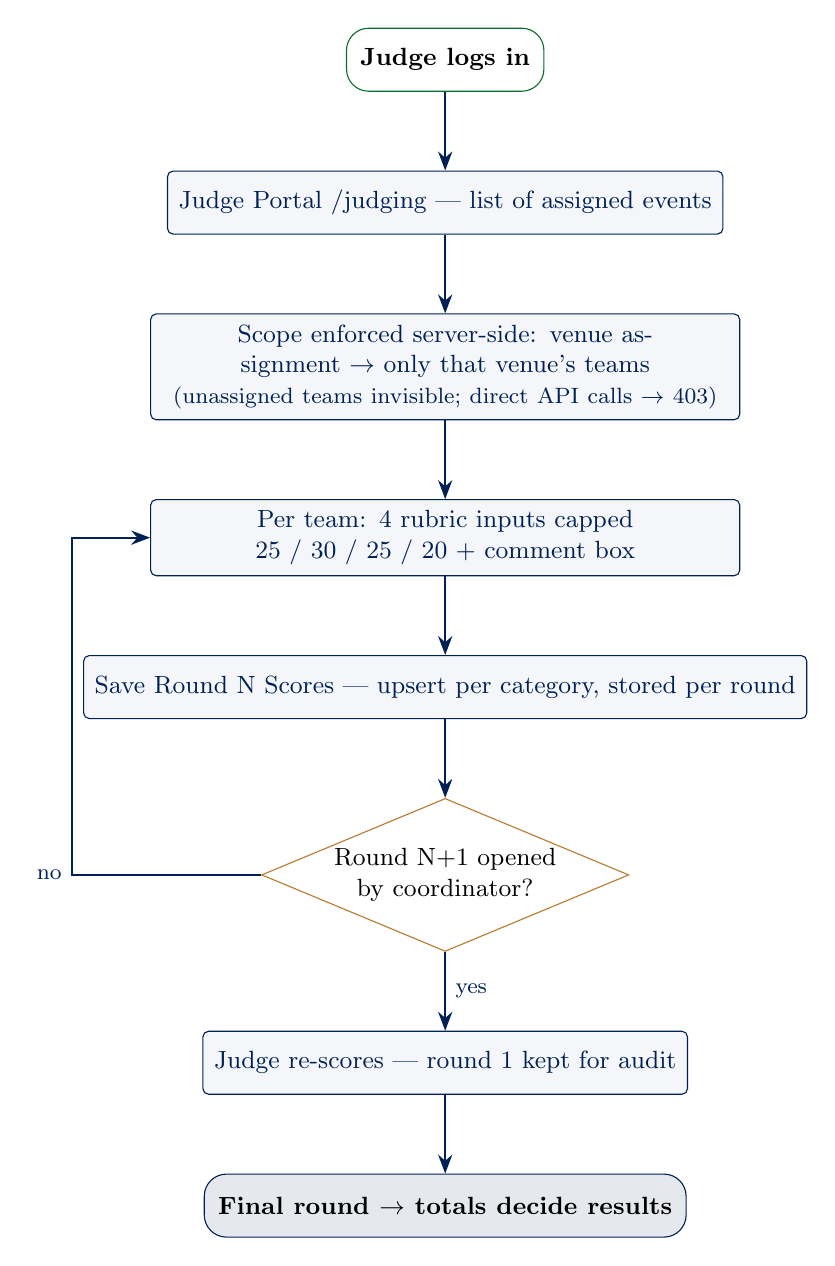
\begin{tikzpicture}[node distance=13mm]
  \node[start] (login) {Judge logs in};
  \node[box, below=10mm of login] (portal) {Judge Portal /judging --- list of assigned events};
  \node[box, below=10mm of portal, text width=72mm] (scope) {Scope enforced server-side: venue assignment $\rightarrow$ only that venue's teams\\\footnotesize (unassigned teams invisible; direct API calls $\rightarrow$ 403)};
  \node[box, below=10mm of scope, text width=72mm] (rubric) {Per team: 4 rubric inputs capped 25 / 30 / 25 / 20 + comment box};
  \node[box, below=10mm of rubric] (save) {Save Round N Scores --- upsert per category, stored per round};
  \node[decision, below=10mm of save] (next) {Round N+1 opened\\by coordinator?};
  \node[box, below=10mm of next] (revisit) {Judge re-scores --- round 1 kept for audit};
  \node[end, below=10mm of revisit] (final) {Final round $\rightarrow$ totals decide results};
  \draw[arrow] (login) -- (portal);
  \draw[arrow] (portal) -- (scope);
  \draw[arrow] (scope) -- (rubric);
  \draw[arrow] (rubric) -- (save);
  \draw[arrow] (save) -- (next);
  \draw[arrow] (next) -- node[right, font=\footnotesize]{yes} (revisit);
  \draw[arrow] (revisit) -- (final);
  \draw[arrow] (next.west) -- ++(-24mm,0) node[left, font=\footnotesize]{no} |- (rubric.west);
\end{tikzpicture}
\end{center}

\section*{6. Data Model}
\begin{center}
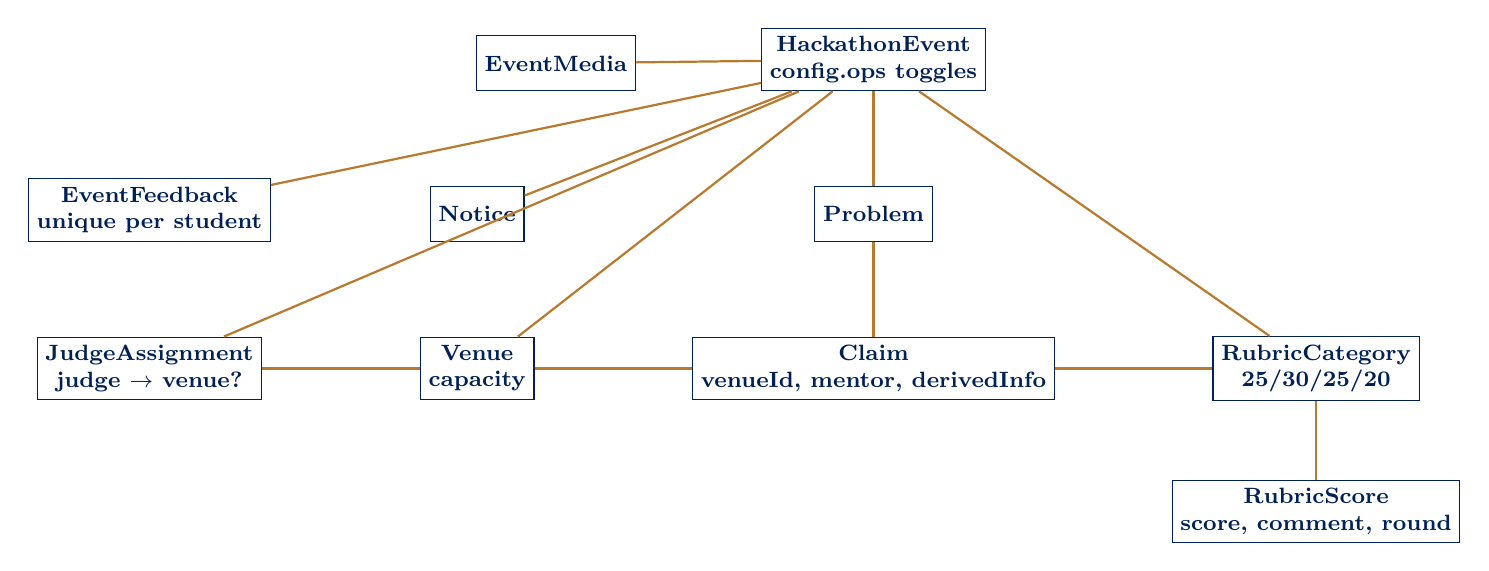
\begin{tikzpicture}[node distance=18mm and 22mm]
  \node[entity] (ev) {HackathonEvent\\\footnotesize config.ops toggles};
  \node[entity, below=12mm of ev] (prob) {Problem};
  \node[entity, below=12mm of prob] (claim) {Claim\\\footnotesize venueId, mentor, derivedInfo};
  \node[entity, right=20mm of claim] (rubric) {RubricCategory\\\footnotesize 25/30/25/20};
  \node[entity, below=10mm of rubric] (score) {RubricScore\\\footnotesize score, comment, round};
  \node[entity, left=20mm of claim] (venue) {Venue\\\footnotesize capacity};
  \node[entity, left=20mm of venue] (jass) {JudgeAssignment\\\footnotesize judge $\rightarrow$ venue?};
  \node[entity, above=12mm of venue] (notice) {Notice};
  \node[entity, above=12mm of jass] (fb) {EventFeedback\\\footnotesize unique per student};
  \node[entity, above=12mm of notice, xshift=10mm] (media) {EventMedia};
  \draw[rel] (ev) -- (prob);
  \draw[rel] (ev) -- (venue);
  \draw[rel] (ev) -- (jass);
  \draw[rel] (ev) -- (notice);
  \draw[rel] (ev) -- (fb);
  \draw[rel] (ev) -- (media);
  \draw[rel] (ev) -- (rubric);
  \draw[rel] (prob) -- (claim);
  \draw[rel] (claim) -- (rubric);
  \draw[rel] (rubric) -- (score);
  \draw[rel] (venue) -- (claim);
  \draw[rel] (venue) -- (jass);
\end{tikzpicture}
\end{center}

\section*{7. Key Rules Enforced}
\begin{itemize}[leftmargin=6mm, itemsep=1mm]
  \item \textbf{One team per student per event} --- duplicate submissions rejected (409).
  \item \textbf{Members must be verified registered students} --- UID checked against active users; duplicate UIDs in the DB are deduped (uid is not unique).
  \item \textbf{PPT lock Sunday 23:59:59 IST} --- submissions and registration freeze together; the portal displays \emph{Registration closes} as the lock time.
  \item \textbf{Scoring caps} --- every category is capped at its weight (25/30/25/20 $\rightarrow$ 100). Overrides and judge saves both enforce it (400).
  \item \textbf{Overrides only during JUDGING} --- after CLOSED, scoring is locked (403).
  \item \textbf{Venue capacity} --- bulk assignment is transactional and rejects over-capacity (409).
  \item \textbf{Rounds} --- scores are stored per round; the final round is authoritative, earlier rounds retained for audit.
  \item \textbf{Feedback} --- opens only after CLOSED, one entry per student (409 on repeat).
  \item \textbf{Media} --- typed uploads with size limits (REPORT $\le$20MB PDF, PHOTO $\le$10MB, VIDEO $\le$100MB); stored in MinIO and served through the auth-gated proxy.
  \item \textbf{Notices} --- visible to every visitor of the event page; pinned notices float to the top.
\end{itemize}

\vfill
{\footnotesize\color{navy!60} TCET CoE-Main --- internal documentation. Dev environment build (2026-08-14). All flows verified end-to-end on the dev portal.}
\end{document}
